% Data for this project is from numerous sources
% Specrtra Data:
%	+ MillerResearchPlots.obj (Origin File)  in Measurements/PS_LiF.
%		- There is a note in that folder containing information about
%		the orginal voltage and gain for these samples.
% 		- The Intrisinic Efficiency, MLLD and other derived parameters
%		are contained within this folder.
% Simulation Data:
%	+ MillerResearchPlots.obj (Origin File)  in Simulation/EnergyDepsotion.
%%%%%%%%%%%%%%%%%%%%%%%%%%%%%%%%%%%%%%%%%%%%%%%%%%%%%%%%%%%%%%%%%%%%%%%%%%%%
%                                                                          %
%                                 PREAMBLE                                 %
%                                                                          %
%%%%%%%%%%%%%%%%%%%%%%%%%%%%%%%%%%%%%%%%%%%%%%%%%%%%%%%%%%%%%%%%%%%%%%%%%%%%
%\documentclass[confrence]{IEEEtran}
\documentclass[draftcls,onecolumn]{IEEEtran}

%%%%%%%%%%%%%%%%%%%%%%%%%%%%%%%%%%%%%%%%%%%%%%%%%%%%%%%%%%%%%%%%%%%%%%%%%%%
%                                                                         %
%                                 PREAMBLE                                %
%                                                                         %
%%%%%%%%%%%%%%%%%%%%%%%%%%%%%%%%%%%%%%%%%%%%%%%%%%%%%%%%%%%%%%%%%%%%%%%%%%%

%% PACKAGES
\usepackage[]{lineno}
%\linenumbers
\usepackage[usenames,dvipsnames]{xcolor}
\usepackage{microtype}
\usepackage[obeyDraft]{todonotes}
\usepackage{fancyvrb}
\VerbatimFootnotes
\usepackage{algorithmic}

%% GRAPHICS RELATED
\usepackage{graphicx}
\usepackage[outdir=./tmp/]{epstopdf}
\graphicspath{{../images/}{./}{./tmp/}}
\DeclareGraphicsExtensions{.eps, .pdf, .jpeg, .png,}

%% CPATION SETUP
\usepackage{float}
\usepackage{caption}
\usepackage{subcaption}
\captionsetup{belowskip=12pt,aboveskip=4pt}


%% BIBLIOGRAPHY
\bibliographystyle{ieeetr}

%% UNITS
\usepackage{siunitx}

%% EQUATIONS
\usepackage{amsmath}
%\numberwithin{equation}{section}

%% HYPERLINKS
\usepackage[debug]{hyperref}

%%%%%%%%%%%%%%%%%%%%%%%%%%%%%%%%%%%%%%%%%%%%%%%%%%%%%%%%%%%%%%%%%%%%%%%%%%%
%                                                                         %
%                             Listing Setup                               %
%                                                                         %
%%%%%%%%%%%%%%%%%%%%%%%%%%%%%%%%%%%%%%%%%%%%%%%%%%%%%%%%%%%%%%%%%%%%%%%%%%%
\usepackage{listings}
\lstset{ %
    language=C++,
    basicstyle=\footnotesize\ttfamily,
    numbers=left,
    numberstyle=\tiny\color{gray},
    stepnumber=2,
    numbersep=5pt,
    backgroundcolor=\color{white},
    showspaces=false,
    showstringspaces=false,
    showtabs=false,
    frame=single,
    rulecolor=\color{black},
    tabsize=2,
    breaklines=true,
    breakatwhitespace=false,
    title=\lstname,
    keywordstyle=\color{blue},
    commentstyle=\color{OliveGreen},
    stringstyle=\color{orange}
}
\DeclareCaptionFont{white}{\color{white}}
\DeclareCaptionFormat{listing}{\colorbox[cmyk]{0.43, 0.35, 0.35, 0.01}{\parbox{\dimexpr\textwidth-2\fboxsep\relax}{#1#2#3}}}
\captionsetup[lstlisting]{format=listing,labelfont=white,textfont=white,singlelinecheck=false,margin=0pt,font={bf,footnotesize}}
%\lstnewenvironment{code}[1][]%
%{ \noindent\minipage{\linewidth}
%	\lstset{#1}
%}
%{\endminipage}
%% USER COMMANDS
\usepackage{isotope}
\newcommand{\iso}{\isotope}
\newcommand{\figurewidth}{\textwidth}
\newcommand{\micron}{$\mu$m}


\sisetup{per-mode=symbol,detect-all}
\usepackage{xfrac}
\sisetup{alsoload=binary}
\DeclareSIUnit\roetgen{R}
\DeclareSIUnit\eV{\electronVolt}
\DeclareSIUnit\count{count}
\DeclareSIUnit\rem{rem}
\DeclareSIUnit\in{in}
\DeclareSIUnit\cps{\count\per\second}
\DeclareSIUnit\cpsngcf{\count\per\second\per\nano\gram\iso[252]{Cf}}

%%%%%%%%%%%%%%%%%%%%%%%%%%%%%%%%%%%%%%%%%%%%%%%%%%%%%%%%%%%%%%%%%%%%%%%%%%%%
%                                                                          %
%                               START OF DOCUMENT                          %
%                                                                          %
%%%%%%%%%%%%%%%%%%%%%%%%%%%%%%%%%%%%%%%%%%%%%%%%%%%%%%%%%%%%%%%%%%%%%%%%%%%%
\newcommand{\papertitle}{Control of Secondary Electron Energy Deposition in Thin Polymeric Films for Neutron-Photon Discrimination}
\begin{document}
\title{\papertitle}
\author{Laurence~F.~Miller,~Matthew~J.~Urffer,~and~Andrew~Mabe%
	\thanks{L. F. Miller and M. Urffer is with the Department of Nuclear Engineering, University of Tennessee, Knoxville, TN 37916 USA email: (lfmiller@utk.edu, murffer@utk.edu).}%
	\thanks{A. Mabe is with the Department of Chemistry, University of Tennessee, Knoxville, TN 37916 USA email: amabe1@utk.edu}%
	\thanks{Manuscript received \textbf{DATE}; revised \textbf{DATE}}%
	\thanks{This works was supported by the Domestic Nuclear Detection Office (DNDO) through award 003387891.
Any opinions, findings, and conclusions or recommendations expressed in this material are those of the authors and do not necessarily reflect the views of DNDO.}}

\markboth{IEEE TRANSACTIONS ON NUCLEAR SCIENCE,~VOL.~00,~NO.~0,~\textbf{DATE}}%
{Miller \MakeLowercase{\textit{et al.}}: \papertitle}

\maketitle
\begin{abstract}
Alternative neutron detection technologies are required to replace the current \iso[3]{He} based Radiation Portal Monitors.
Replacement technologies must fulfill two basic criteria; 1) a neutron detection efficiency, and 2) the performance of the detector should not suffer in the the presence of a strong gamma field.
The difference in the energy deposition mechanics from a charge particle (originating from the fission products of a neutron interaction) and the Compton scattered electrons from a gamma interaction allows for the effective discrimination between neutrons and gammas based on energy deposition.
Polymeric films containing \iso[6]{LiF} ranging from \SI{15}{\um} to \SI{1}{\cm} where fabricated and tested for their neutron count rate above a lower level discriminator necessary to meet the gamma intrinsic efficiency set forth by PNNL.
The energy deposition in the films was also simulated with GEANT4 and compared to the measured pulse height spectra.
\end{abstract}

\begin{IEEEkeywords}
Energy Deposition, Detectors, Monte-Carlo Simulation, GEANT4
\end{IEEEkeywords}

\IEEEpeerreviewmaketitle

%%%%%%%%%%%%%%%%%%%%%%%%%%%%%%%%%%%%%%%%%%%%%%%%%%%%%%%%%%%%%%%%%%%%%%%%%%%
%                                                                         %
%                               INTRODUCTION                              %
%                                                                         %
%%%%%%%%%%%%%%%%%%%%%%%%%%%%%%%%%%%%%%%%%%%%%%%%%%%%%%%%%%%%%%%%%%%%%%%%%%%
\section{Introduction}
\label{sec:Intro}
The Department of Homeland Security (DHS) continues to fund research (through the Domestic Nuclear Detection Office (DNDO)) to detect radioactive material that could potentially be used to cause significant economic loss and loss or life.  
The current technology used in Radiation Portal Monitors (RPMs) for detecting neutrons emitted from special nuclear material uses a rapidly diminishing resource, \iso[3]{He}, that cannot be economically replaced. 
As a result a number of alternative detection systems continue to be investigated with the most viable including: boron trifluoride filled proportional detectors, boron-lined proportional detectors, \iso[6]{Li} loaded scintillation glass fiber detectors, and \iso[6]{Li} plus scintillator-coated wavelength-shifting fiber detectors\cite{pnnl_18471,kouzes_neutron_2010}.  

Pacific Northwest National Lab (PNNL) along with the DNDO have developed a set of specifications that that replacement RPMs must meet \cite{kouzes_neutron_2010, kouzes_neutron_1999}. 
In particular 1) an absolute neutron detection efficiency greater than \SI{2.5}{\cps} at \SI{2}{\meter} for a defined moderated  source, 2) an intrinsic gamma-neutron detection efficiency of one in a million, and 3) a gamma absolute rejection ratio for neutrons stating that the performance of the detector should not change by more than 10\% in a \SI{10}{\milli\roetgen\per\hour} gamma field (Table \ref{tab:DHSCritera}).
\begin{align}
  \label{eqn:garrn}
  GARRn = \frac{ \epsilon_{abs,\gamma n}}{\epsilon_{abs,n}}
\end{align}
\begin{table}
  \centering
	\caption{Replacement Portal Monitor Criteria}
	\begin{tabular}{m{2.5cm} m{2.5cm} }
	Parameter & Specification \\
	\hline
	\hline
	Absolute neutron detection efficiency & 2.5 cps/ng of \iso[252]{Cf} (in specified test configuration) \\
	Intrinsic gamma-neutron detection efficiency & $ \epsilon_{int,\gamma n}\leq 10^{-6}$ \\
	Gamma absolute rejection ratio for neutrons (GARRn) & $ 0.9 \leq \text{ GARRn }\leq$ 1.1 at 10 mR/h exposure \\
	Cost &  \$ 30,000 per system \\
	\end{tabular}
	\label{tab:DHSCritera}
\end{table}

The absolute neutron detection efficiency $\left (\epsilon_{abs,n} \right )$ is defined as the number of neutron pulses recorded divided by the number of neutrons emitted by the source (with only a neutron source present) as shown in \eqref{eqn:absn}.
\begin{align}
	\label{eqn:absn}
  \epsilon_{abs,n} = \frac{N_{nc}}{N_{ns}}
\end{align}
where:
\begin{itemize}
 \item[] $N_{nc}$ is the neutron count rate, and
 \item[] $N_{ns}$ is the neutron emission rate from the source.
\end{itemize}
DNDO guidelines state that a \iso[252]{Cf} source is to be used for the determination of the absolute neutron detection efficiency \cite{pnnl_18471}.
To reduce the gamma ray flux of \iso[252]{Cf} upon a candidate detector the source is sheilded by at least \SI{0.5}{\cm} of lead\cite{pnnl_18471}.
The neutron spectrum is then moderated by \SI{2.5}{\cm} of polyethylene\cite{pnnl_18471}.
The source is then placed \SI{2}{\meter} from the midpoint of the detector.
The intrinsic gamma-neutron detection efficiency $\left(\epsilon_{int,\gamma n}\right)$  is defined as the number of neutron pulses detected divided by the number of photons striking the detector, thus measuring the response of a neutron detector to the presence of a gamma ray field when no neutron source is present .
This is shown in \eqref{eqn:intGN}
\begin{align}
  \label{eqn:intGN}
  \epsilon_{int,\gamma n} = \frac{N_{pc}}{N_{pi}}
\end{align}
where:
\begin{itemize}
 \item[] $N_{pc}$ is the number of photons that produce counts which are indistinguishable from neutrons per unit time, and 
 \item[] $N_{pi}$ is the neutron of photons incident on the detector per unit time.
\end{itemize}
The intrinsic gamma-neutron detection efficiency is to be measured using either a \iso[192]{Ir}, \iso[137]{Cs}, or \iso[60]{Co} source placed at an appropriate distance so as to produce an exposure rate of \SI{10}{\milli\roetgen\per\hour} at the detector\cite{kouzes_neutron_1999}.
The gamma absolute rejection ratio for neutrons (GARRn) is a parameter that characterizes the detector response in the presence of both a large gamma ray source (\SI{10}{\milli\roetgen\per\hour}) and a \iso[252]{Cf} neutron source (configured as it would be for an absolute neutron detection efficiency measurement).
The GARRn is defined as the absolute neutron detection efficiency in the presence of both sources, divided by the absolute neutron detection efficiency of the neutron detector in the presence of only the neutron source as shown in \eqref{eqn:garrn}\cite{kouzes_neutron_1999}.

You may note from the PNNL summary report \cite{pnnl_18471}  that satisfying intrinsic gamma efficiency is problematic for some of the technologies evaluated.
It is shown in this paper that this problem can be solved for thin films that contain a neutron absorber.
In particular, differences in properties between secondary electrons produced by photon interactions and by charged particles slowing down in layered thin-film neutron detectors can be used to obtain neutron-photon discrimination that is sufficient to satisfy Department of Homeland Security (DHS) criteria for portal monitors.  


%%%%%%%%%%%%%%%%%%%%%%%%%%%%%%%%%%%%%%%%%%%%%%%%%%%%%%%%%%%%%%%%%%%%%%%%%%%
%                                                                         %
%                                 THEORY                                  %
%                                                                         %
%%%%%%%%%%%%%%%%%%%%%%%%%%%%%%%%%%%%%%%%%%%%%%%%%%%%%%%%%%%%%%%%%%%%%%%%%%%
\section{Technical Basis}
Neutron detectors often utilize a material with a large cross section for absorption, such as \iso[6]{Li} or \iso[10]{B}.
When these materials absorb a neutron they usually disintegrate to produce ionized reaction products that in turn transfer their kinetic energy to many electrons.
In the case of $\iso[6]{Li}\left(n,\iso[3]{H}\right)\alpha$ the fission energy is distributed between a triton of energy \SI{2.73}{\mega\eV} and an alpha of energy \SI{2.05}{\mega\eV}.
Compton scattering is the predominant interaction mechanism for the \SI{1.173}{\mega\eV} and \SI{1.332}{\mega\eV} from \iso[60]{Co} in which a photon interacts with a single electron and has the ability to transfer a majority of the photons energy \cite{turner_atoms_2008}.
%The difference in the transfer of kinetic energy from charged particles to electrons and from photon interactions to electrons may be exploited to maximize the discrimination between neutron and photon interactions in a detector.  
For a particular material and neutron absorber, one can optimize the detector geometry to maximize the energy deposited in scintillation material by charged particles relative to the energy deposited by photon interactions. 
This in turn permits one to maximize the recorded neutron interaction rate relative to recorded photon interaction rates by setting a lower level discriminator (LLD) above a threshold associated with energy deposited in the detector by photons.  
As the LLD is increased, the efficiency for detecting neutrons is diminished; however, the intrinsic efficiency for detecting neutrons relative to photons is dramatically increased. 

The maximum kinetic energy of an electron from a Compton scattering event with an impingement \iso[60]{Co} source is \SI{1.117}{\mega\eV} (for the \SI{1.332}{\mega\eV} gamma). 
In polystyrene with a denisty of \SI{1}{\gram\per\cm\cubed}, the range of the maximum electron from Compton scattering is around \SI{4.5E3}{\um}\cite{berger_estar_2005}.
If elastic scattering between the alpha, triton and electrons is assumed the maximum kinetic energy of an electron is \SI{1.097}{\kilo\eV} for the alpha particle and \SI{1.986}{\kilo\eV} for the triton\cite{turner_atoms_2008}.
The range of the electron from a gamma interaction is more than \num{1E3} times greater than the range of electrons from an alpha or triton (Table \ref{tab:BasicEDepOutline}).
Therefore, it is more likely that the electrons generated by the alpha and the triton deposit significantly more of their energy in a thin film than the electron from a gamma.
This is also reflected in the stopping power, where the reaction product secondary electrons have a stopping power 40 times that of the secondary electrons from a gamma \cite{berger_estar_2005}.
\begin{table}[ht]
  \caption{Electron Energy, Range, and Stopping Power\protect\cite{berger_estar_2005,turner_atoms_2008}}
	\centering
	\begin{tabular}{c | c S c}
	{Electron Parent} & {Electron Energy} & {Total Stopping Power} & {CSDA Range} \\
	 &  & \si{\mega\eV \cm\squared \per \gram} & \si{\gram\per\cm\squared} \\
	\hline
	\hline
	{gamma}  & \SI{1.12}{\mega\eV} & 1.79 & $\ge$~\num{4.48E-1} \\
	{triton} & \SI{1.99}{\kilo\eV} & 75.1 & $\le$~\num{2.55E-4} \\
	{alpha}  & \SI{1.10}{\kilo\eV} & 113  & $\le$~\num{2.55E-4} \\
	\end{tabular}
  \label{tab:BasicEDepOutline}
	% See pg. 87 of Matthew's lab notebook for the calculation
\end{table}

%%%%%%%%%%%%%%%%%%%%%%%%%%%%%%%%%%%%%%%%%%%%%%%%%%%%%%%%%%%%%%%%%%%%%%%%%%%
%                                                                         %
%                                   METHODS                               %
%                                                                         %
%%%%%%%%%%%%%%%%%%%%%%%%%%%%%%%%%%%%%%%%%%%%%%%%%%%%%%%%%%%%%%%%%%%%%%%%%%%
\section{Methods}
\label{sec:Methods}
The energy deposition of neutrons and gammas was investigated for polymeric films containing \iso[6]{Li} for thickness ranging from \SI{15}{\um} to \SI{1}{\cm}.
The pulse height spectra of these samples were measured at the University of Tennessee's characterization laboratory from a moderated neutron source and a \iso[60]{Co} source.
Energy deposition simulations were completed using GEANT4, a modern toolkit for Monte Carlo transport simulation \cite{agostinelli_geant4simulation_2003,allison_geant4_2006}.

\subsection{Fabricated Detector Measurements}
Samples are mounted to a 10 stage photo multiplier tube (PMT) with silicone based optical grease. 
The PMT is attached to a Canberra base (also serving as a preamplifier). 
The PMT's voltage is supplied by a high voltage power supply, with the power being supplied to the preamplifier base by an amplifier.  
The output signal of the base feeds into the amplifier for pulse shaping and amplification. 
The amplified signal is then inputted to an multi-channel analyzer and analog to digitical converter (MCB-ADC), and can then be read using the MAESTRO-32 software. 
A schematic of the setup is shown in Figure \ref{fig:ElectronicsSpectra}.
\begin{figure}
	\centering
	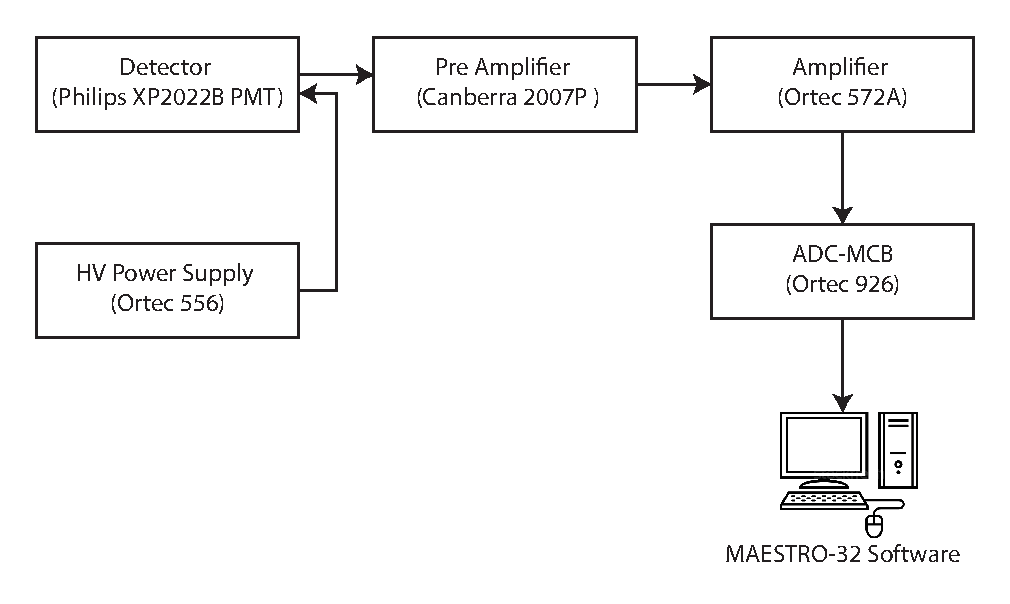
\includegraphics[width=\textwidth]{ElectronicsSpectra}
	\caption{Pulse height measurement electronics}
	\label{fig:ElectronicsSpectra}
\end{figure}

The gamma irridiator fabircated for our research is shown in Fiugre Figure \ref{fig:gammaIrridiator}.
A 100 $\mu$Ci \iso[60]{Co} source is contained in \SI{2}{\in} of steel, with a \SI[fraction-function = \sfrac]{1/8}{\in} thick steel cap.
The detector well is a \SI{4}{\in} outer diameter \SI{14}{\in} pipe that is \SI{1/4}{\in} thick, and \SI{7}{\cm} of foam is used to ensure that the detector rests at a \SI{10}{\milli\roetgen\per\hour} field.
The detector well is surounded by \SI{4}{\in} x \SI{8}{\in} x \SI{2}{\in} lead bricks, which are contained in a an outer steel outer box \SI{14}{\in} x \SI{12}{\in} x \SI{12}{\in}.
\begin{figure}[ht]
	\centering
	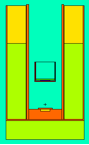
\includegraphics[height=4cm]{GammaIrridiatorMCNPXRender.png}
	\caption{MCNPX Rendering of Gamma Irridiator}
	\label{fig:gammaIrridiator}
\end{figure}
The gamma intrinsic efficiency of the sample is calculated by integrating the measured spectra, $p(x)$, as a function of a mathematical lower level channel discriminator $MLLD$ setting and dividing by the incident photon fluence, $\Phi$, as shown in \eqref{eqn:mlld}.
The incident photon fluence was calculated with MCNPX (a Monte Carlo transport code\cite{pelowitz_mcnpx_????}) and confirmed by measurements.
At a distance of \SI{10.2}{\cm} from the source the dose rate was measured to be \SI{10}{\milli\rem\per\hour}, and the simulated dose rate was \SI{10.3}{\milli\rem\per\hour}.
\SI{28}{\cm} from the source the measured dose rate was \SI{2}{\milli\rem\per\hour} which is in good agreement of the simulated dose rate of \SI{1.80}{\milli\rem\per\hour}.
The intrinsic efficiency necessary to meet the criteria is determined by the $MLLD$ (corresponding to a channel) for which $\epsilon_{int,\gamma} \left(MLLD\right) \le \si{1E-6}$.
\begin{align}
	\label{eqn:mlld}
	\epsilon_{int,\gamma} \left(MLLD\right) = \frac{\int_{MLLD}^\infty p(x)dx}{\Phi} 
\end{align}

The neutron irridiator is a custom built facility that contains a \SI{0.59}{\ug}\iso[252]{Cf}  source encased in 2” blocks of high density polyethylene (HDPE), to moderate the \iso[252]{Cf} spectrum.
The HDPE box is approximately \SI{20}{\in}  long, \SI{12}{\in} wide, and \SI{14}{\in} tall.
There are two detector \SI{1/16}{\in} thick acrylic detectors wells, one surrounded by a \SI{1/16}{\in} cadmium to shield out thermal neutrons, and the other surrounded by \SI{1/16}{\in} of lead to shield out a similar amount of gammas as the cadmium well.
The \iso[252]{Cf} source is surrounded by stainless steel, which in turn is contained within a \SI{2}{\in} diameter, \SI{1/2}{\in} thick, \SI{5}{\in} tall lead vessel. 
Figure \ref{fig:neutronIrridiator} is an MCNPX rendering of the neutron irridiator.
\begin{figure}[ht]
	\centering
	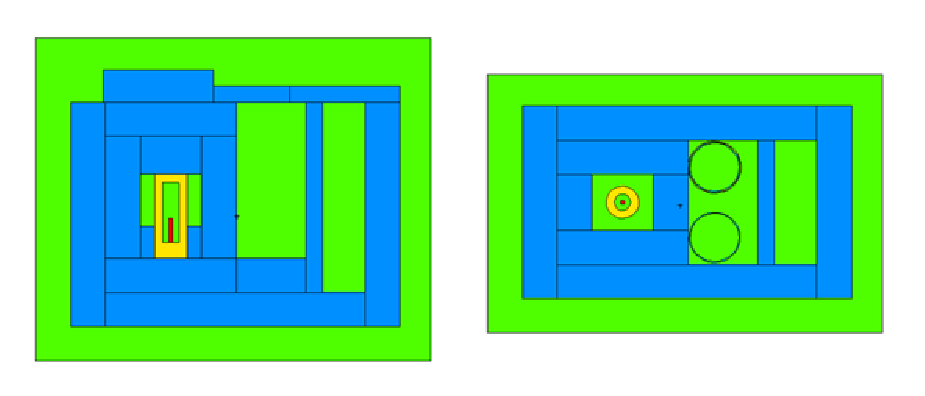
\includegraphics[width=\textwidth]{NeutronIrridiator_MCNP.eps}
	\caption{MCNPX Rendering of Neutron Irridiator}
	\label{fig:neutronIrridiator}
\end{figure}
The lead well measures the response of neutron of all energies, while the cadmium well measures the responses of fast neutrons.
The two responses are then subtracted to yield the thermal neutron response.

MCNPX modeling of the neutron irridiator caluclate an interaction rate for a 1" diameter \SI{2}{\mm} thick \iso[6]{Li} glass (GS20) of 423 interactions per second as of December 1st, 2012.
The observed count rate of GS20 measured on December 1st, 2012 was \SI{428}{\cps}. 
Polymeric films had a simulated neturon interaction rate within 15\% of the observed count rate.
Therefore, even though this source is not the same configuration as specified by PNNL, neutronic simulations in MCNPX can be used to relate the interactions to a simulated interaction rate for a detector mocked up according the the PNNL specifications encased in the RPM8 footprint.

\subsection{Detector Simulation}
The energy deposition from neutron and gamma interactions was simulated with the GEANT4 toolkit \cite{agostinelli_geant4simulation_2003}.
The detector geometry was represented as a single layer of neutron absorbing thin polymeric film mounted on top of a non-scintillating material (PMMA).
The initial events for runs where chosen by setting up a particle gun for thermal (\SI{0.025}{\eV}) neutrons upon the detector and for both gammas resulting from a \iso[60]{Co} decay.
The Livermore physics were used as the ionization module, extending the standard electro-magnetic physics down to \SI{1}{\kilo\eV}.
High performance, data driven hadronic modules were used in order to simulate the neutron and the subsequent reaction product transport.

The simulation was validated by reproducing the single collision energy loss for water as well as comparing spectra shapes and averages of simulated spectra to the measured spectra.
The single collision energy loss spectra for water that was simulated is shown in Figure \ref{fig:SingleCollisionELossWater}.
In general there was excellent agreement between the simulated energy spectra and a previously published spectra\cite{turner_comparative_1982}, with the simulated spectra having much better resolution than the reference did not.
It is thought that this is due to the water model in GEANT4 having better cross sections than the previously published spectra.
\begin{figure}[ht]
  \centering
  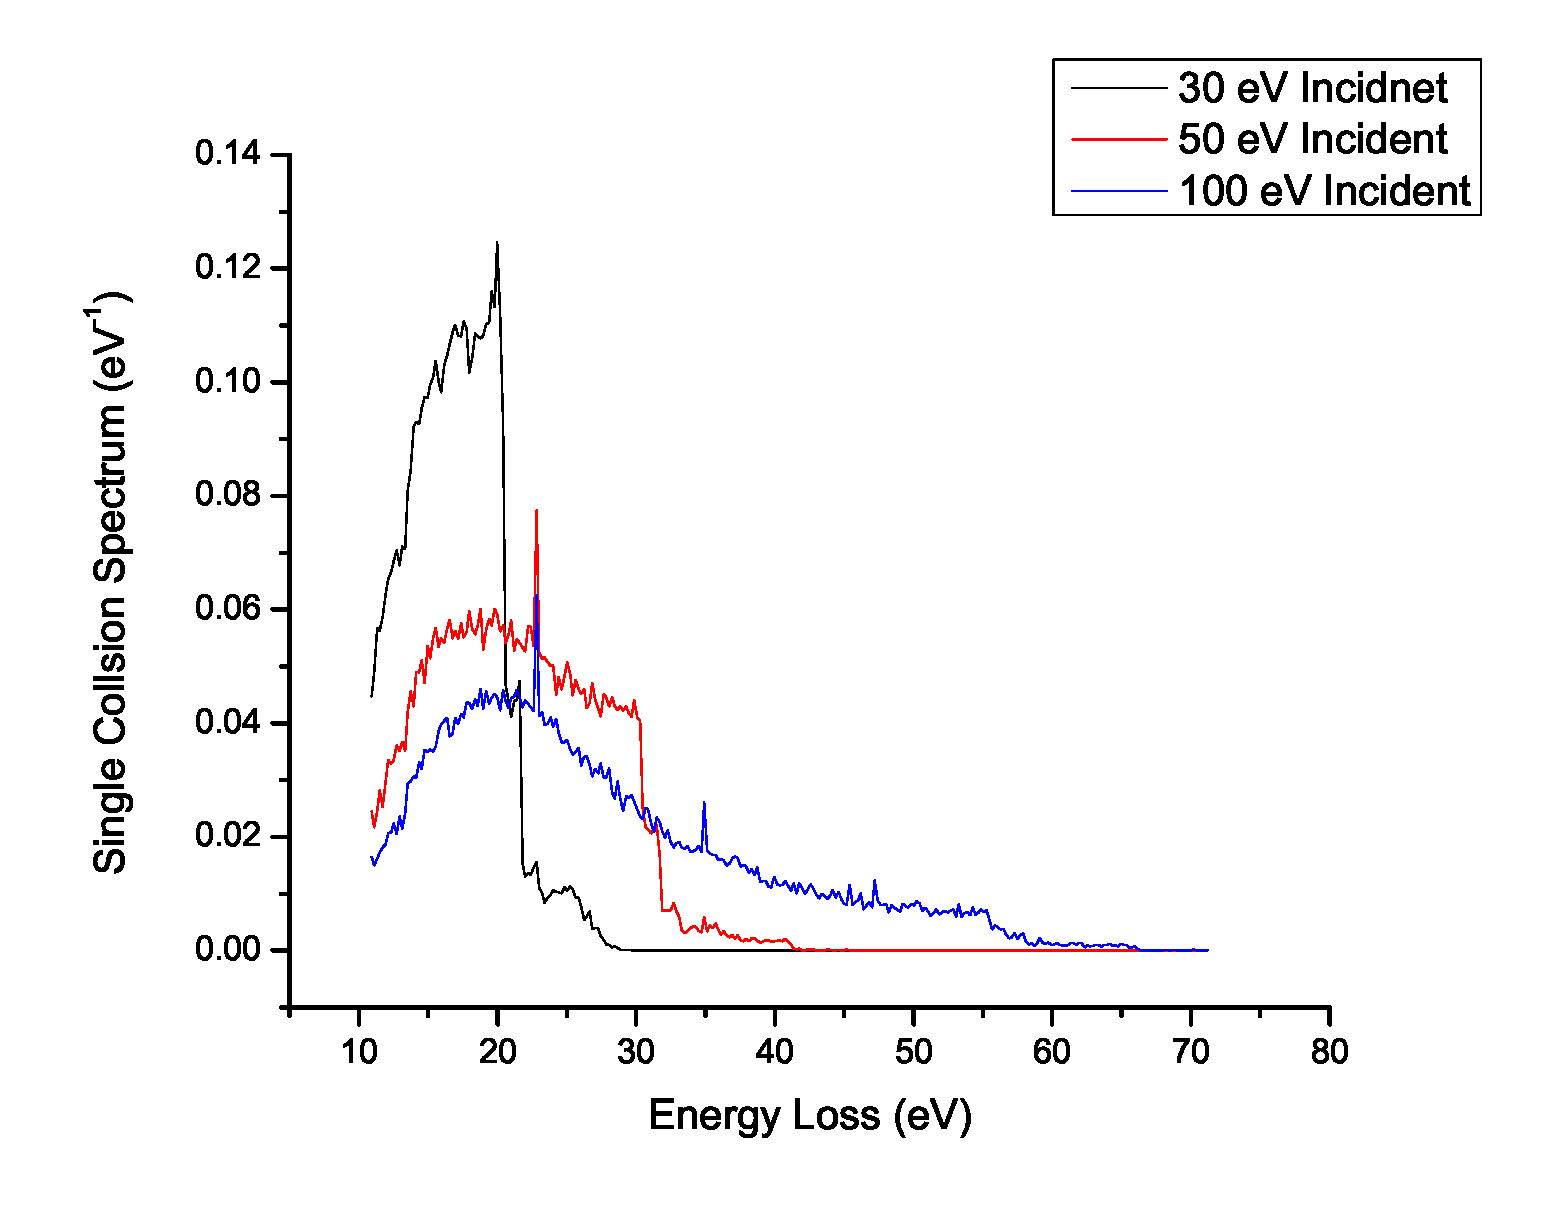
\includegraphics[width=\textwidth]{SingleCollisionEnergyLoss_300bins}
  \caption{Single Collision Energy Loss of Water. The simulated energy spectra matches that of Turner\cite{turner_comparative_1982}.}
	\label{fig:SingleCollisionELossWater}
\end{figure}

The validity of the GEANT4 simulation is determined by comparing the spectra shapes of measured spectra to simulated energy deposition.
Figure \ref{fig:spectraComparisonGamma} shows the comparison between the simulated energy deposition per incident photon from a \iso[60]{Co} source and the measured pulse height spectra from the \iso[60]{Co} irridiator per incident photon.
The energy calibration on the upper axis of the measured spectran was completed by finding the channel number at a given intrisinic efficiency and the corresponding energy at that intrisinic efficiency.
The energy of this feature on the measured spectra was then compared to the energy on the simulated spectra, with all of the values being within 10\%.
\begin{figure*}[ht]
	\centering
	\begin{subfigure}[b]{0.45\textwidth}
    		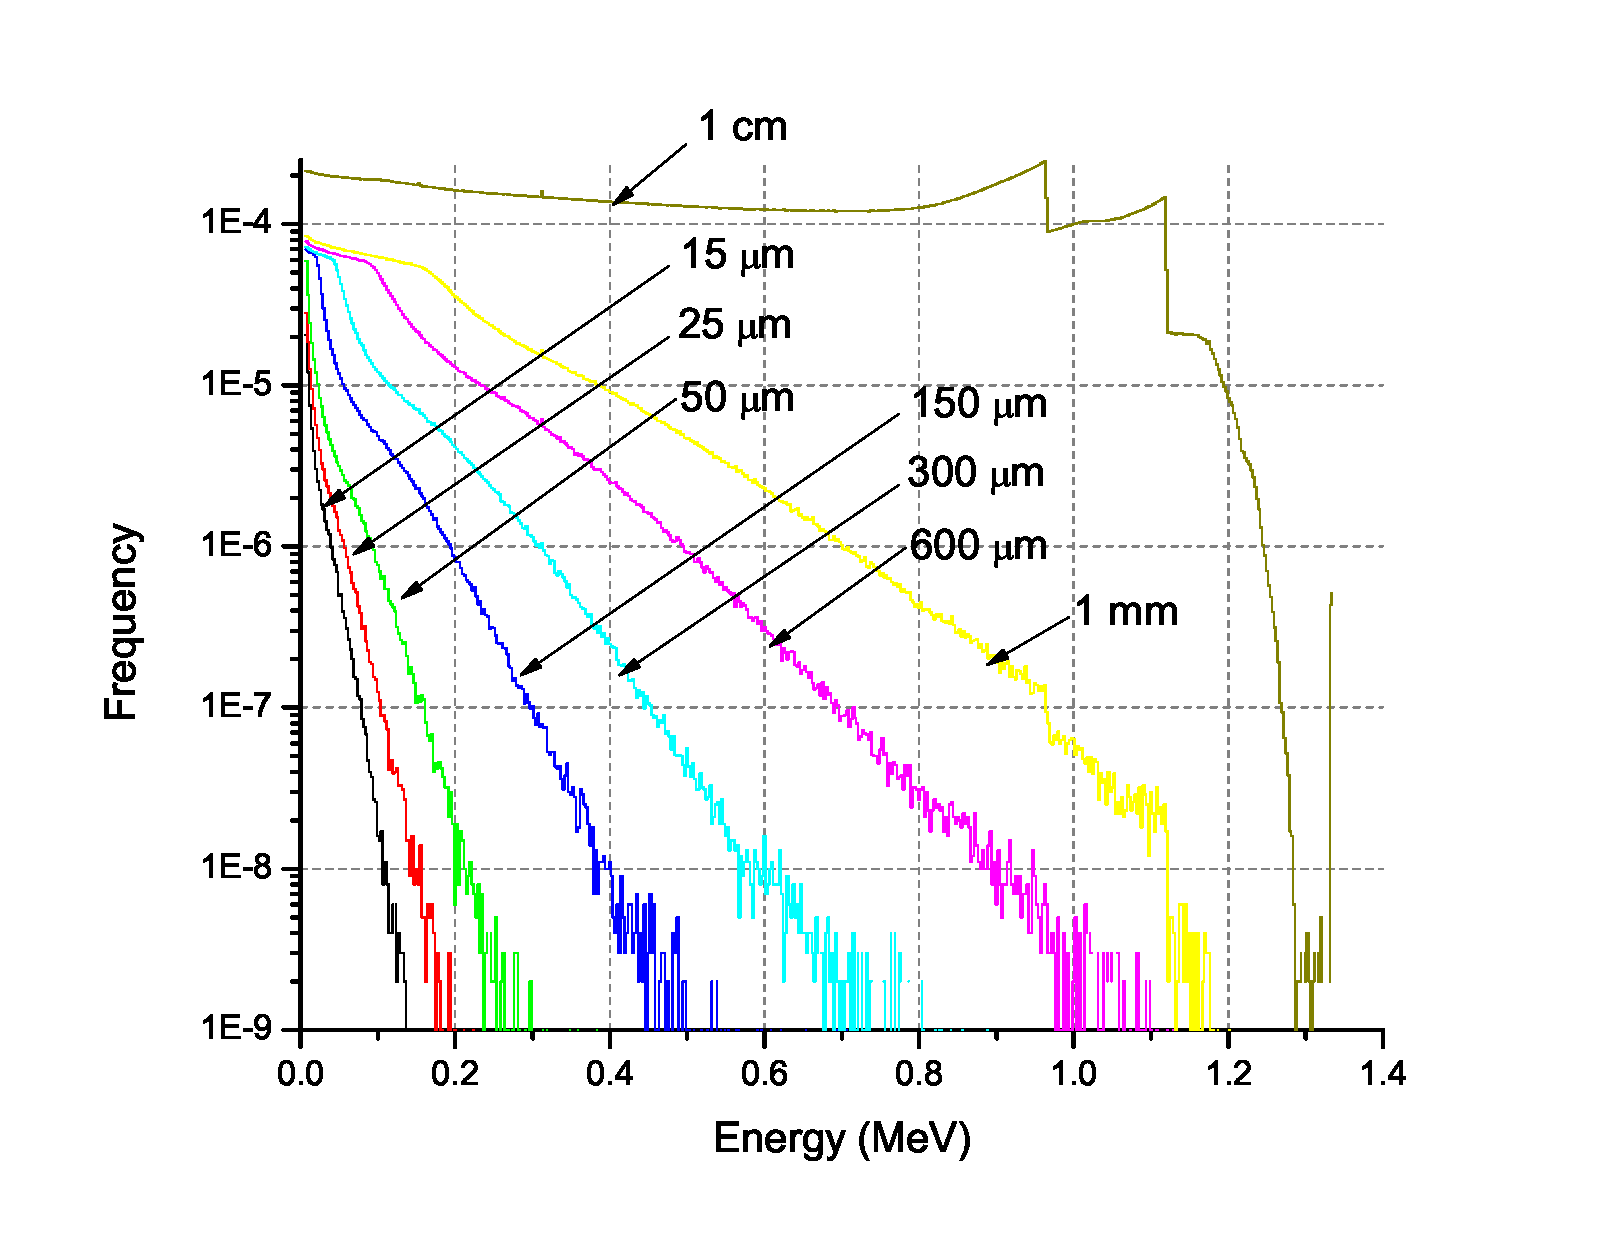
\includegraphics[width=\textwidth]{PS_EDepSim_Co60}
		\caption{GEANT4 Simulated Energy Deposition}
	\end{subfigure}%
	~
	\begin{subfigure}[b]{0.45\textwidth}
    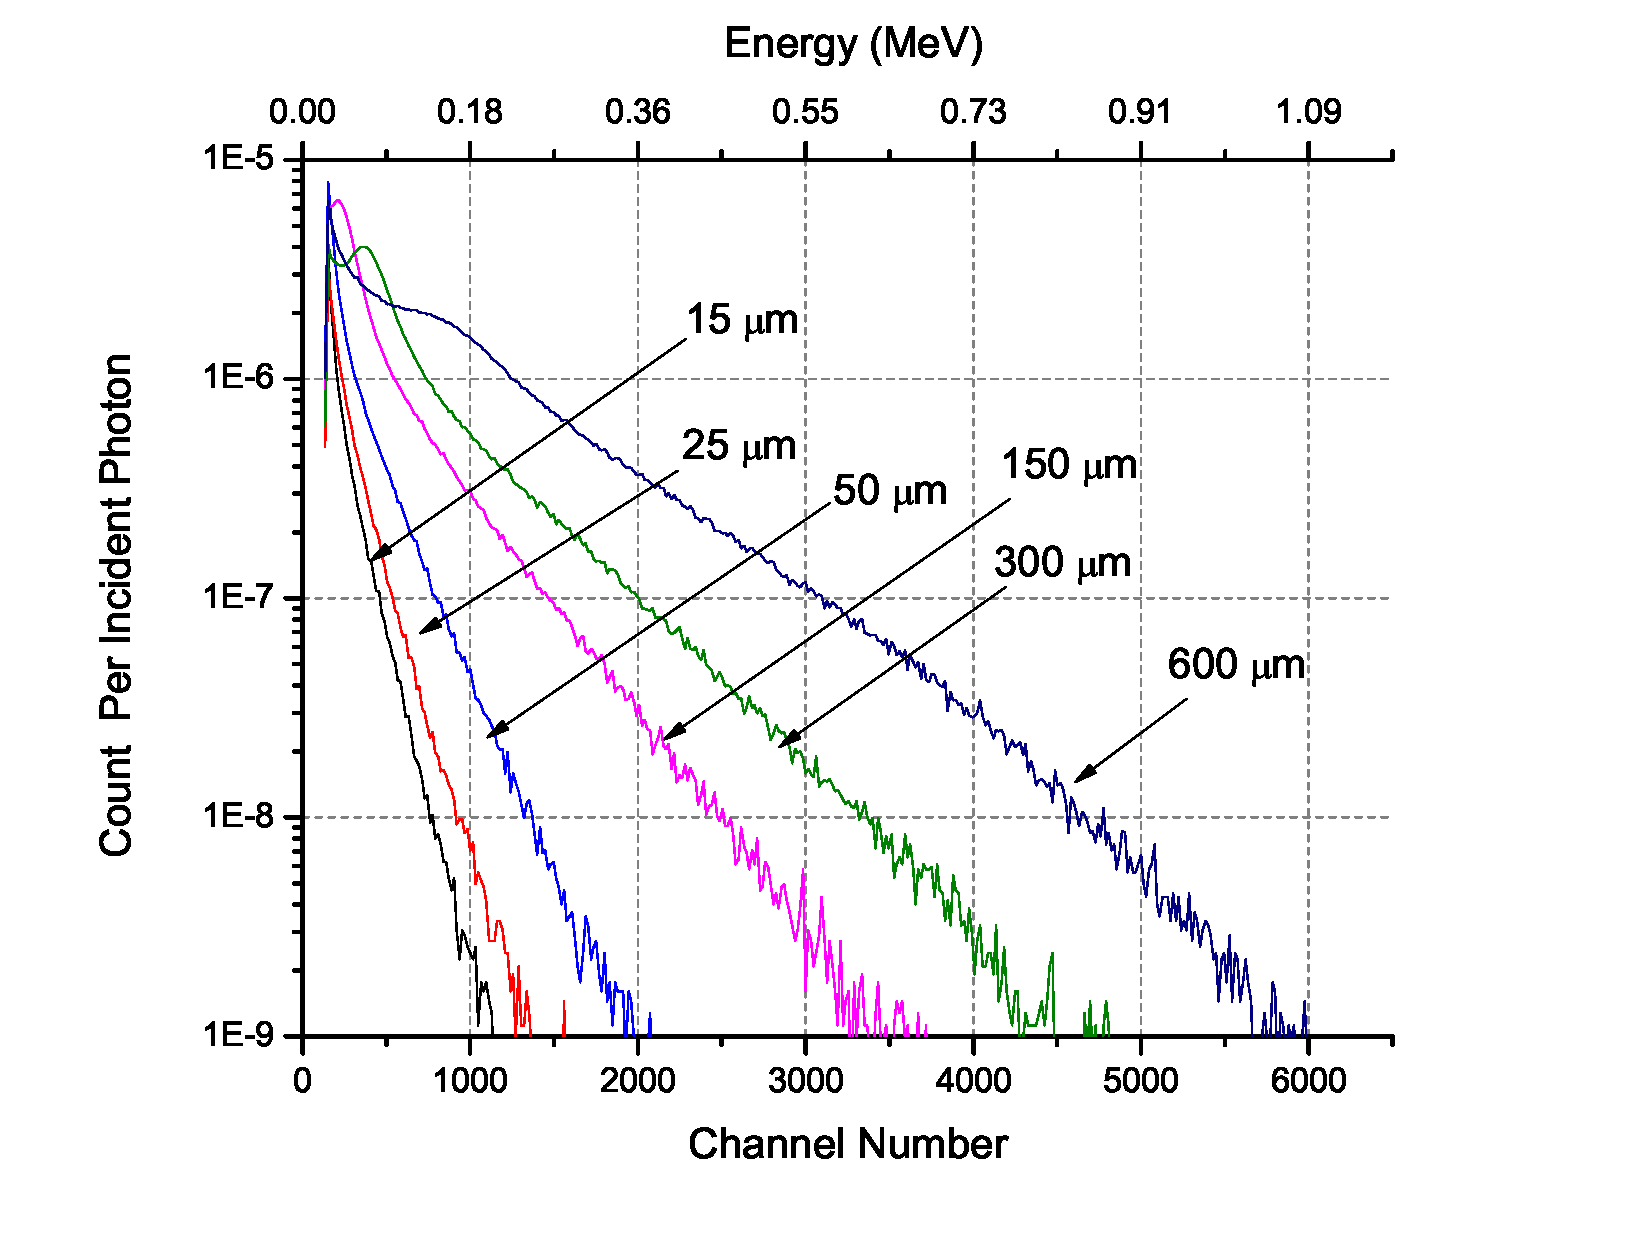
\includegraphics[width=\textwidth]{PS_GammaCR-Binned-FluxNorm_20LiF_5PPO}
		\caption{Measured Pulse Height Spectra}
	\end{subfigure}%
	\caption{Comparison of the energy deposition and binned pulse height spectra for validation. The spectra have the same shape, indicating agreement. The fabricated films greater than \SI{600}{\um} were of poor optical quality and therefore their results are not shown.}
	\label{fig:spectraComparisonGamma}
\end{figure*}
The average energy deposition and average pulse height are shown in Figure \ref{fig:EDepLightYield}. 
With the average energy deposition on the left axis and the average light yield (pulse height) on the right axis, it is possible to compare the measurement and the simulation and agreement is observed.
\begin{figure*}[ht]
	\centering
	\begin{subfigure}[b]{0.45\textwidth}
    		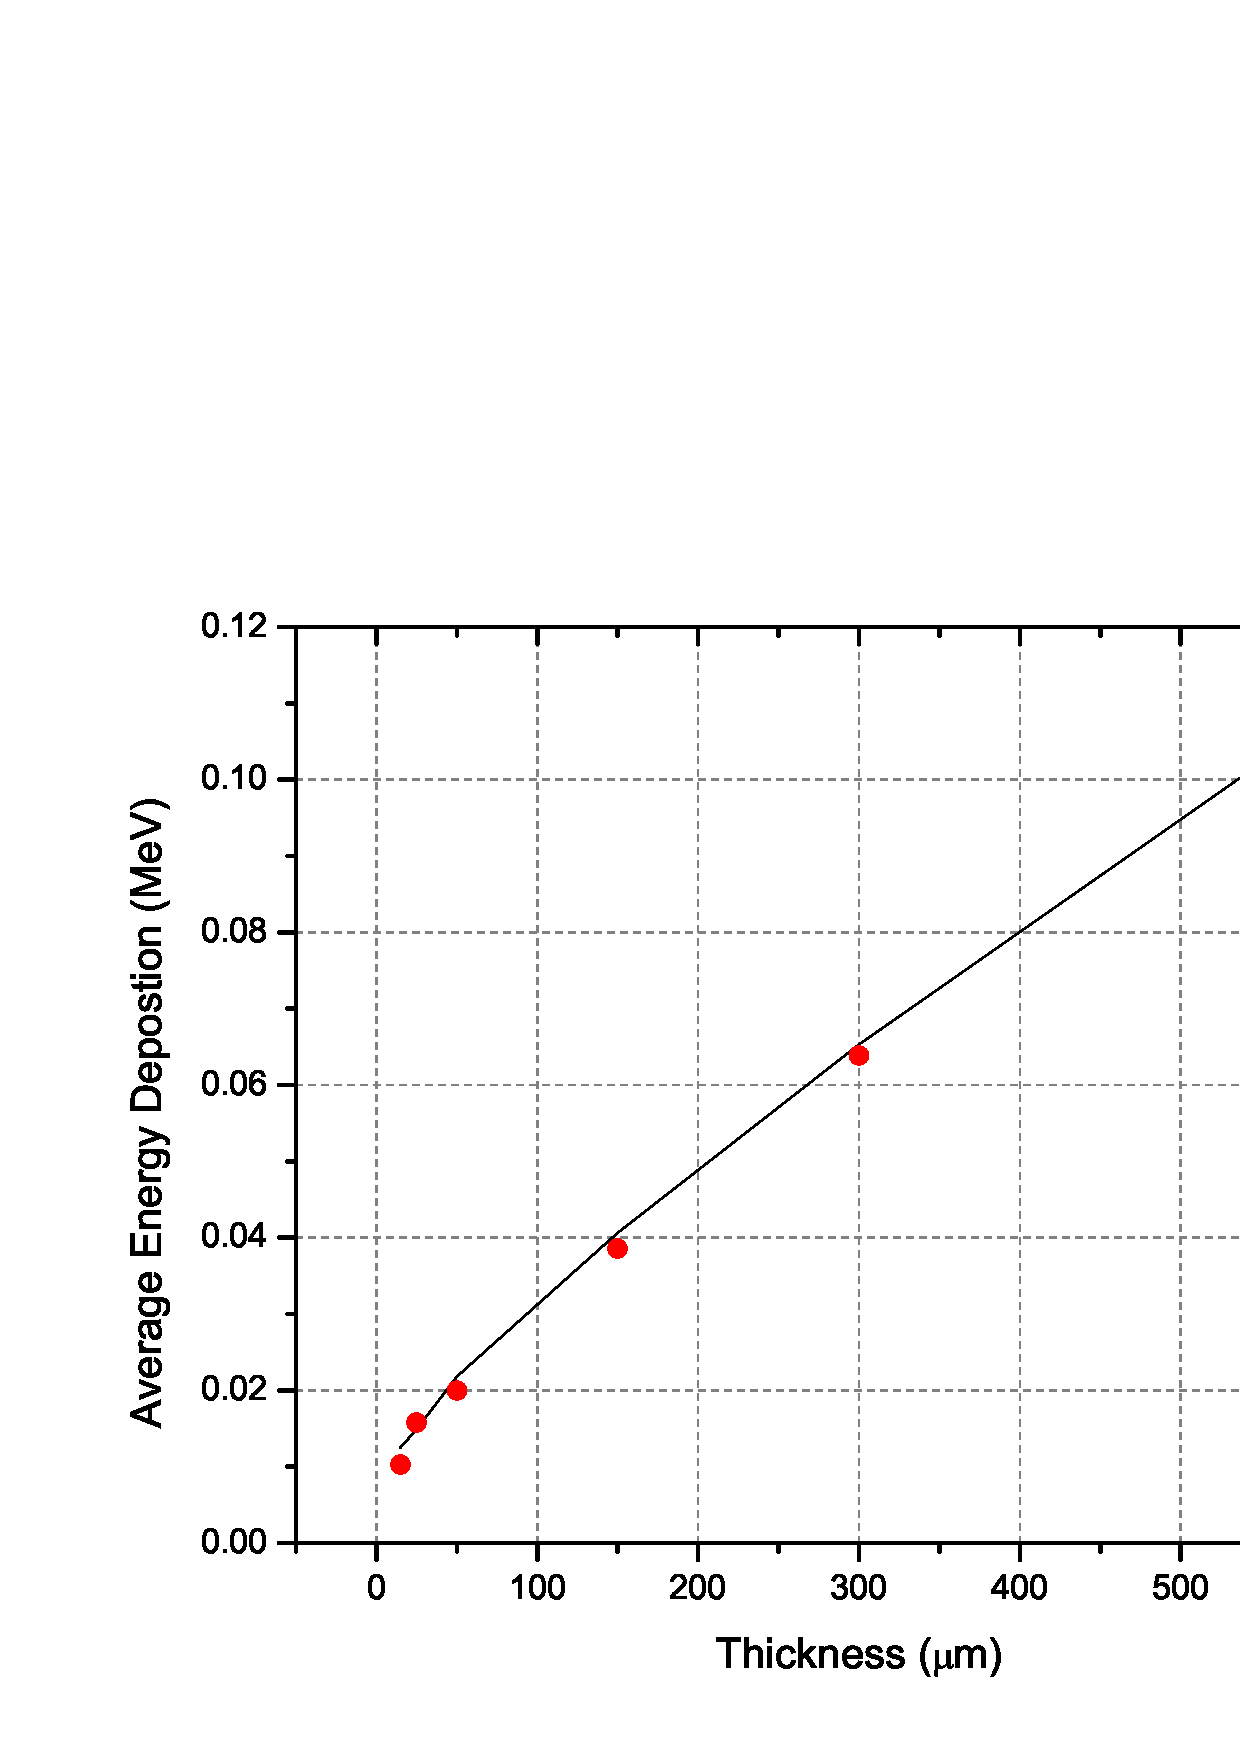
\includegraphics[width=\textwidth]{G4EDep_LightYield_Co60}
		\caption{Gamma (\iso{Co}{60})}
	\end{subfigure}%
	~
	\begin{subfigure}[b]{0.45\textwidth}
    		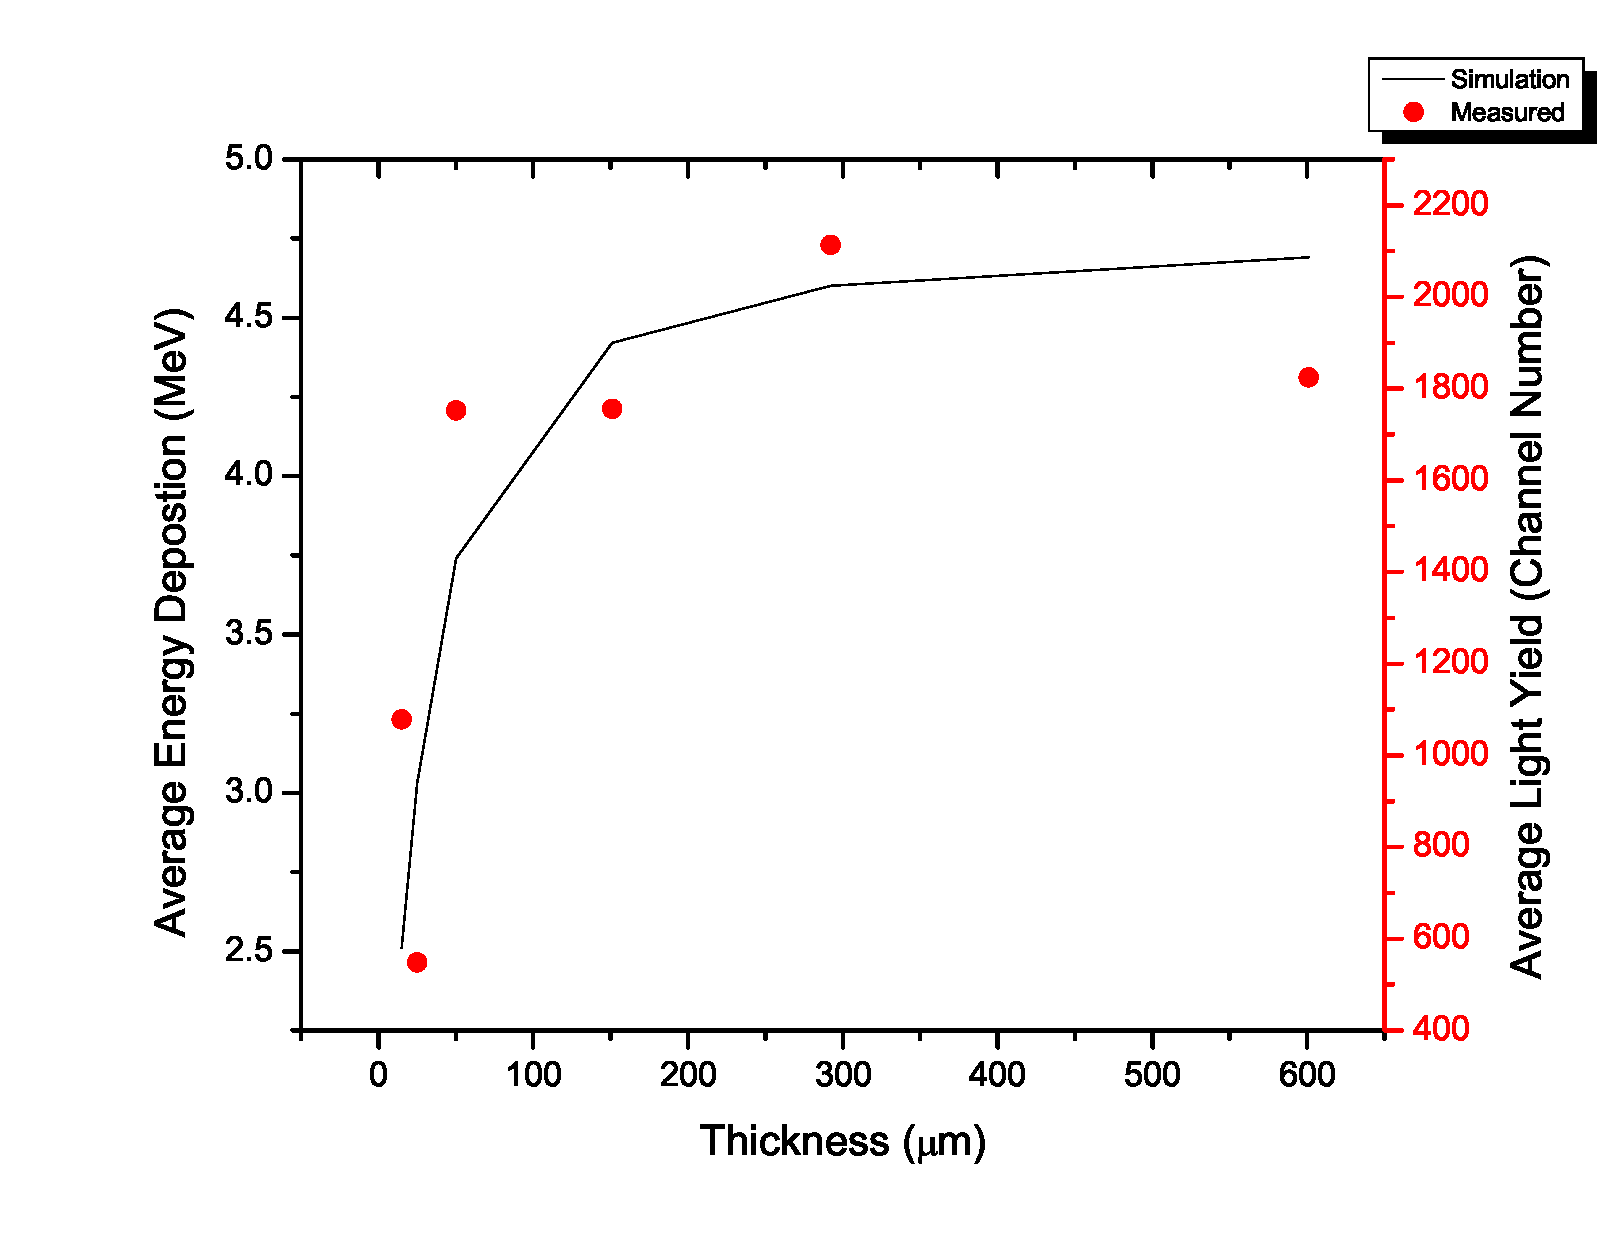
\includegraphics[width=\textwidth]{G4EDep_LightYield_Neutron}
		\caption{Neutrons}
	\end{subfigure}%
	\caption{Average Energy Deposition and Measured Light Yield. The solid lines are calculated values and the red dots are measurments.}
	\label{fig:EDepLightYield}
\end{figure*}
%%%%%%%%%%%%%%%%%%%%%%%%%%%%%%%%%%%%%%%%%%%%%%%%%%%%%%%%%%%%%%%%%%%%%%%%%%%
%                                                                         %
%                     RESULTS and ANALYSIS                                %
%                                                                         %
%%%%%%%%%%%%%%%%%%%%%%%%%%%%%%%%%%%%%%%%%%%%%%%%%%%%%%%%%%%%%%%%%%%%%%%%%%%
\section{Results}
\label{sec:Results}
The calculated gamma intrinsic efficiency for six polymeric films along with the neutron response of two of the films in Figure \ref{fig:GammaIntrNeutronCounts}, and the fraction of neutron counts above the MLLD necessary for a given gamma intrinsic efficiency is plotted in Figure \ref{fig:crVsIntEff}.
It is observed that if the films are thin enough (less than \SI{150}{\um}) it is possible to have a significant count rate above the the mathematical lower level discriminator necessary for the pulse height discrimination of one in a million.
This is seen by the \SI{50}{\um} film and the \SI{150}{\um} film having the tail of their neutron spectra above the pulse height discriminator necessary for an intrinsic efficiency of \num{1E-6}.
Table \ref{tab:FractionCRGamma} shows the fraction of neutron count rate that is above the MLLD necessary for $\epsilon_{int,\gamma n} \le \si{1E-6}$.
Films less than \SI{50}{\um} have over 2\% of the counts above the necessary discriminator setting, while thicker films have have a factor of 10 less.
\begin{figure}[ht]
    \centering
    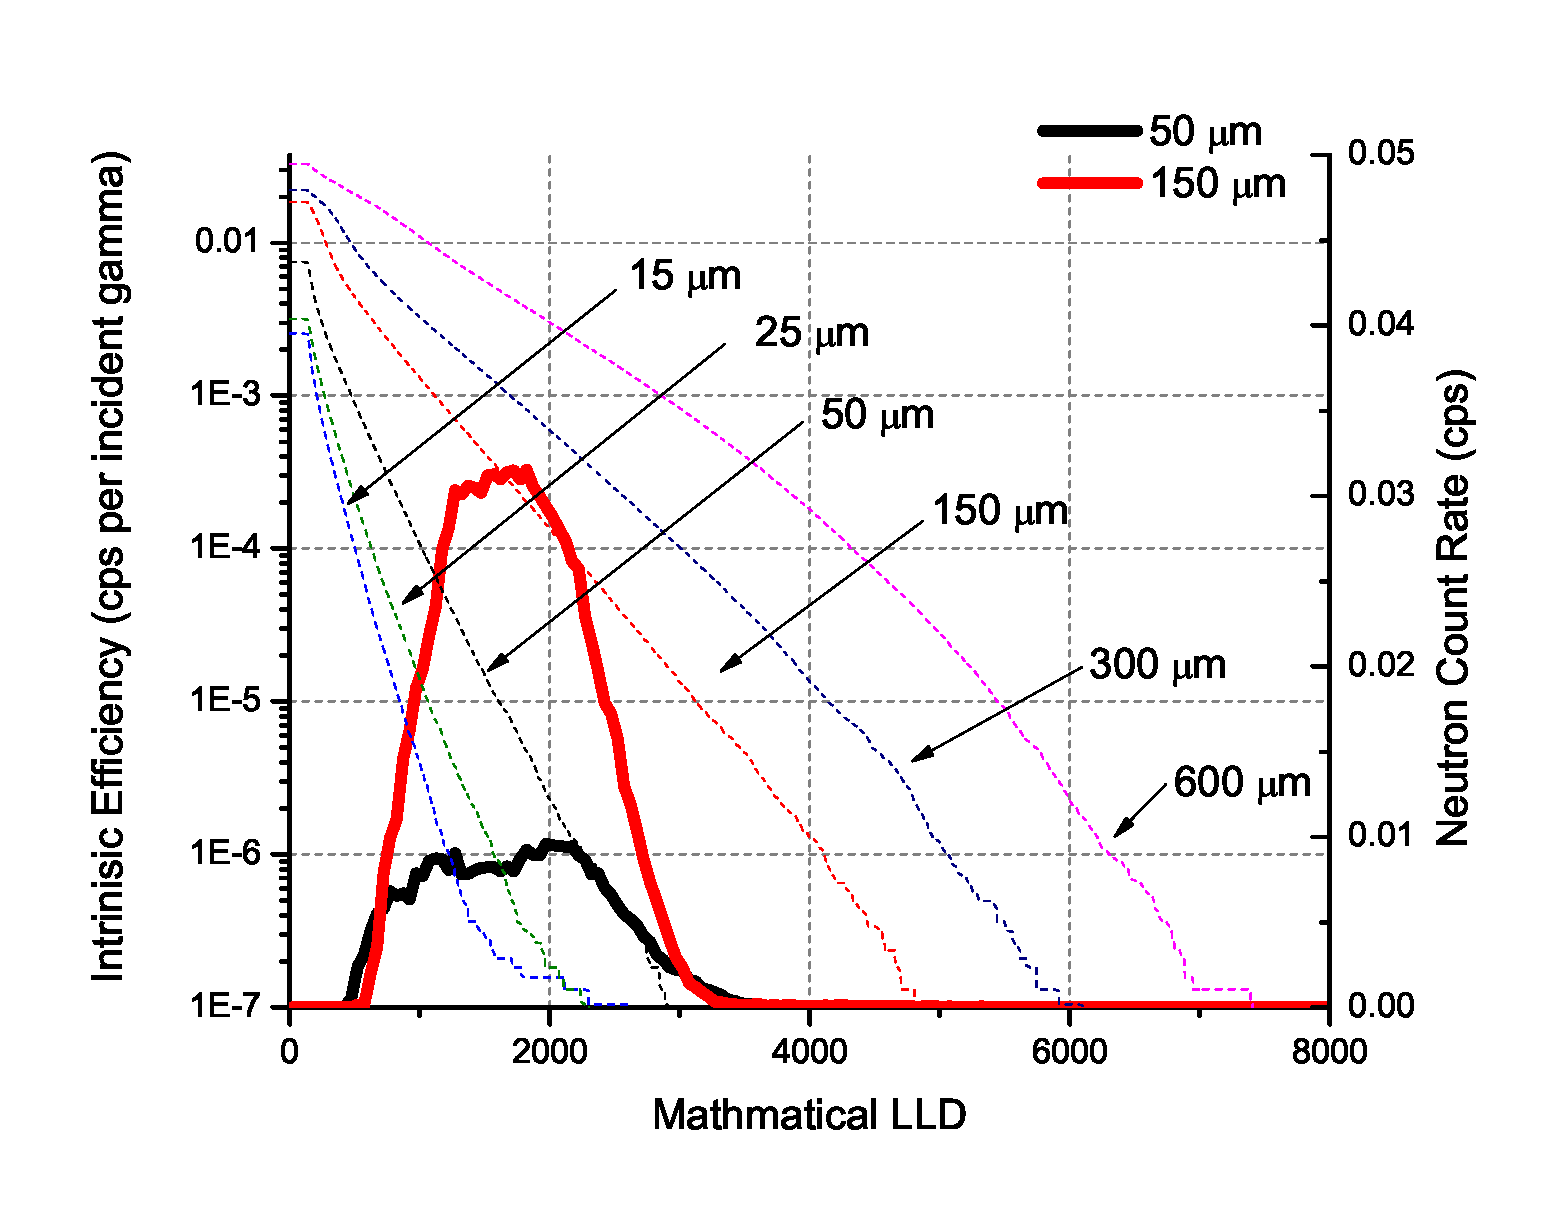
\includegraphics[width=\textwidth]{PS_IntEff_LiF20_PPO5}
    \caption{Gamma intrinsic efficiency (dashed lines) plotted against neutron counts (solid). The gamma spectra has been normalized by the number of incident photons upon the sample, while the neutron spectra has not.}
    \label{fig:GammaIntrNeutronCounts}
\end{figure}
\begin{figure}[ht]
    \centering
    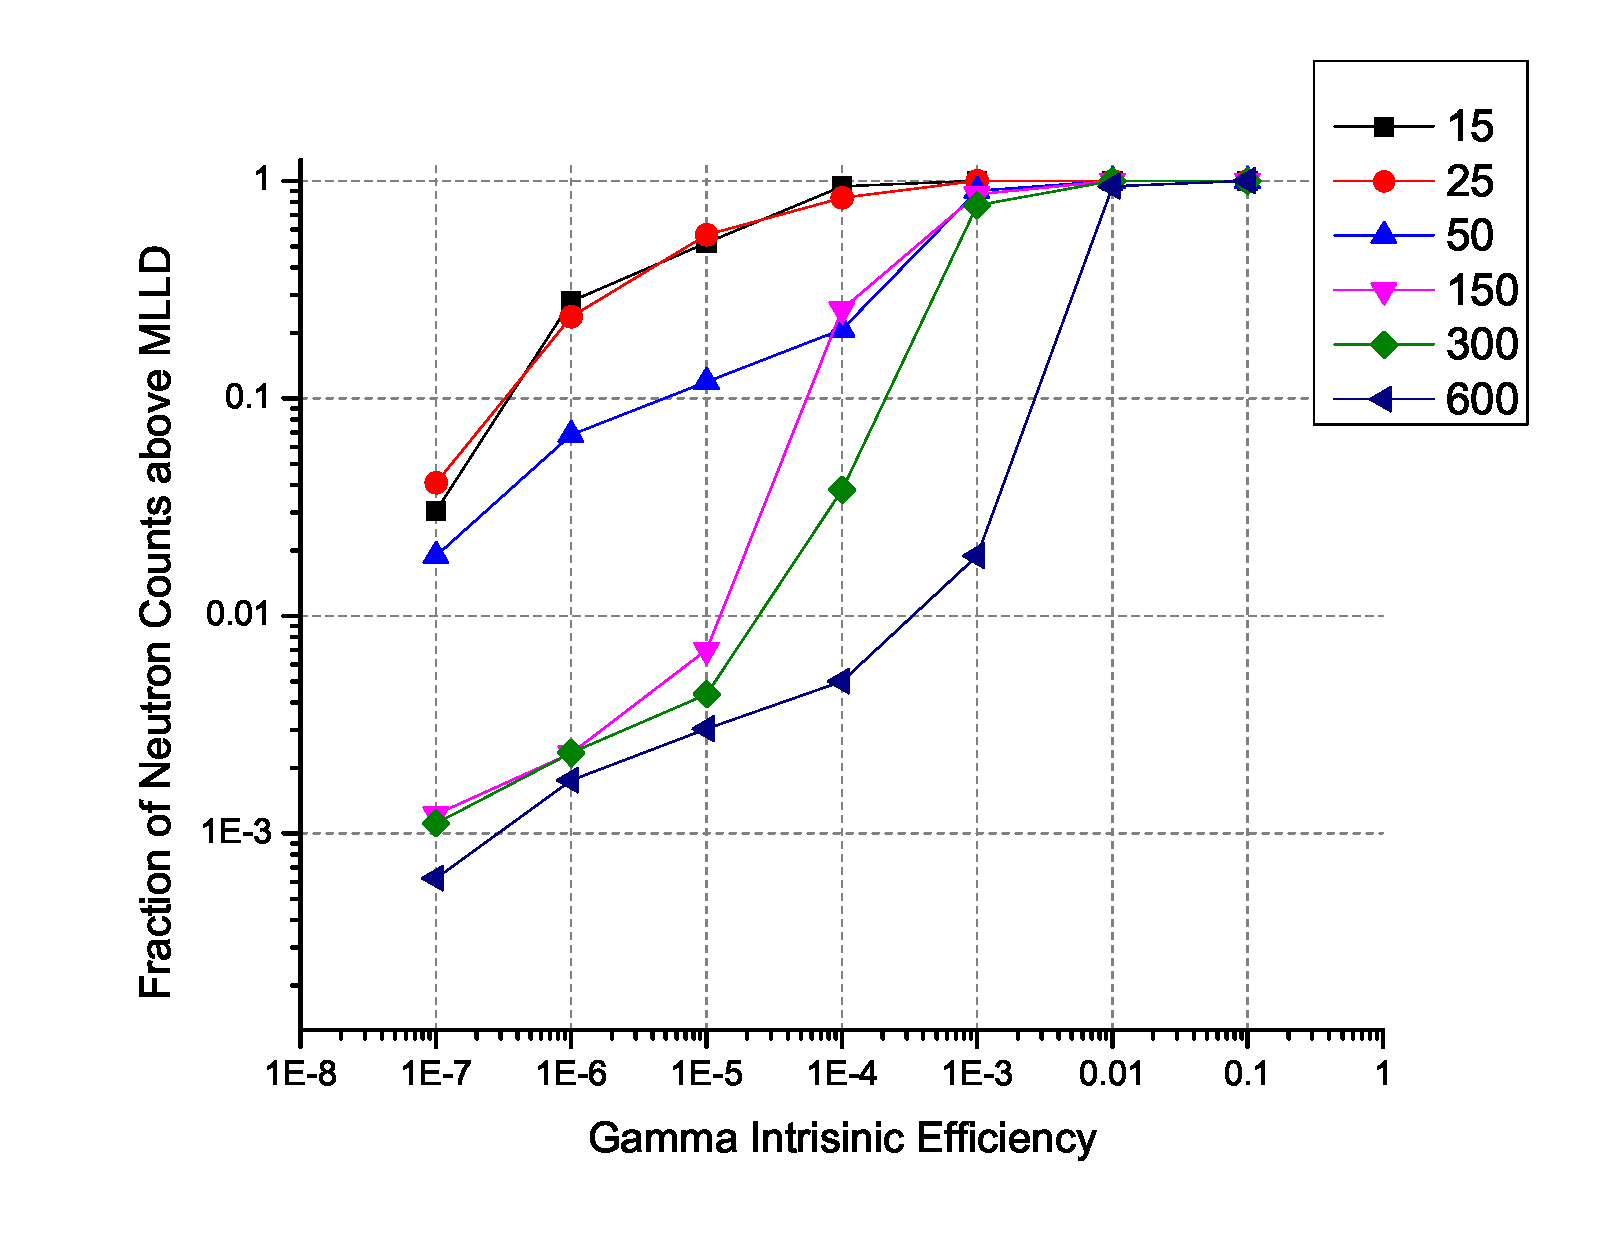
\includegraphics[width=\textwidth]{PS_IntFractionNCR_LiF}
    \caption{Intrinsic efficiency versus neutron count rate. }
    \label{fig:crVsIntEff}
\end{figure}
\begin{table}[]
    \caption{Fraction of Neutron Count Rate Above Discriminator Setting}
	\centering
	\begin{tabular}{c | c}
	Thickness & Neutron Fraction \\
	\hline
	\hline
	\SI{15}{\um} & 0.28 \\
	\SI{25}{\um} & 0.024 \\
	\SI{50}{\um}  & 0.067 \\
	\SI{150}{\um}  & 0.023 \\
	\SI{300}{\um}  & 0.023 \\
	\SI{600}{\um}  & 0.0017 \\
	\end{tabular}
  \label{tab:FractionCRGamma}
\end{table}
In addition it is observed in Figure \ref{fig:GammaIntrNeutronCounts} that for neutrons, thicker films only enhance the resolution of the film and do little to increase the light yield, as most of energy from a neutron event is captured in the film.
The average energy deposited was computed for each thickness and normalized by the incident energy for gammas by the Q-value of the reaction for neutrons, and is presented in Table ~\ref{tab:FractionEDep}.
For thickness greater than \SI{150}{\um} there is little benefit in increasing the thickness of the film in terms of energy deposition by neutrons, since over 90\% of the energy is being deposited in the film.
\begin{table}[ht]
    \caption{Fractional Energy Deposition for Various Thickness}
	\centering
	\begin{tabular}{c | c c}
	Thickness & Gamma Fraction & Neutron Fraction \\
	\hline
	\hline
	\SI{15}{\um} & 0.010 & 0.531 \\
	\SI{25}{\um} & 0.013 & 0.634 \\
	\SI{50}{\um} & 0.017 & 0.782 \\
	\SI{150}{\um} & 0.032 & 0.927 \\
	\SI{300}{\um} & 0.052 & 0.964 \\
	\SI{600}{\um} & 0.087 & 0.982 \\
	\SI{1}{\mm} & 0.130 & 0.989 \\
	\SI{1}{\cm} & 0.425 & 0.998 \\
	\end{tabular}
  \label{tab:FractionEDep}
\end{table}

Figure \ref{fig:simKinE} illustrates the simulated kinetic energy of secondary electrons from Compton scattering and from alpha and triton interactions.
It is observed that kinetic energy of the secondary electrons from the neturon reaction products have prediomantely energies in the kilo-volt range, while the Compton scattering electrons have energies in hundreds of kilovolts range. 
However, it should be noted that there is only one secondary electron from a Compton scattering and multiple secondary electrons from the reaction products.
Figure \ref{fig:ReacProdDist} shows the distrubtion of the number of secondary electrons from the alpha and triton and their kinetic energy.
\begin{figure}[ht]
    \centering
    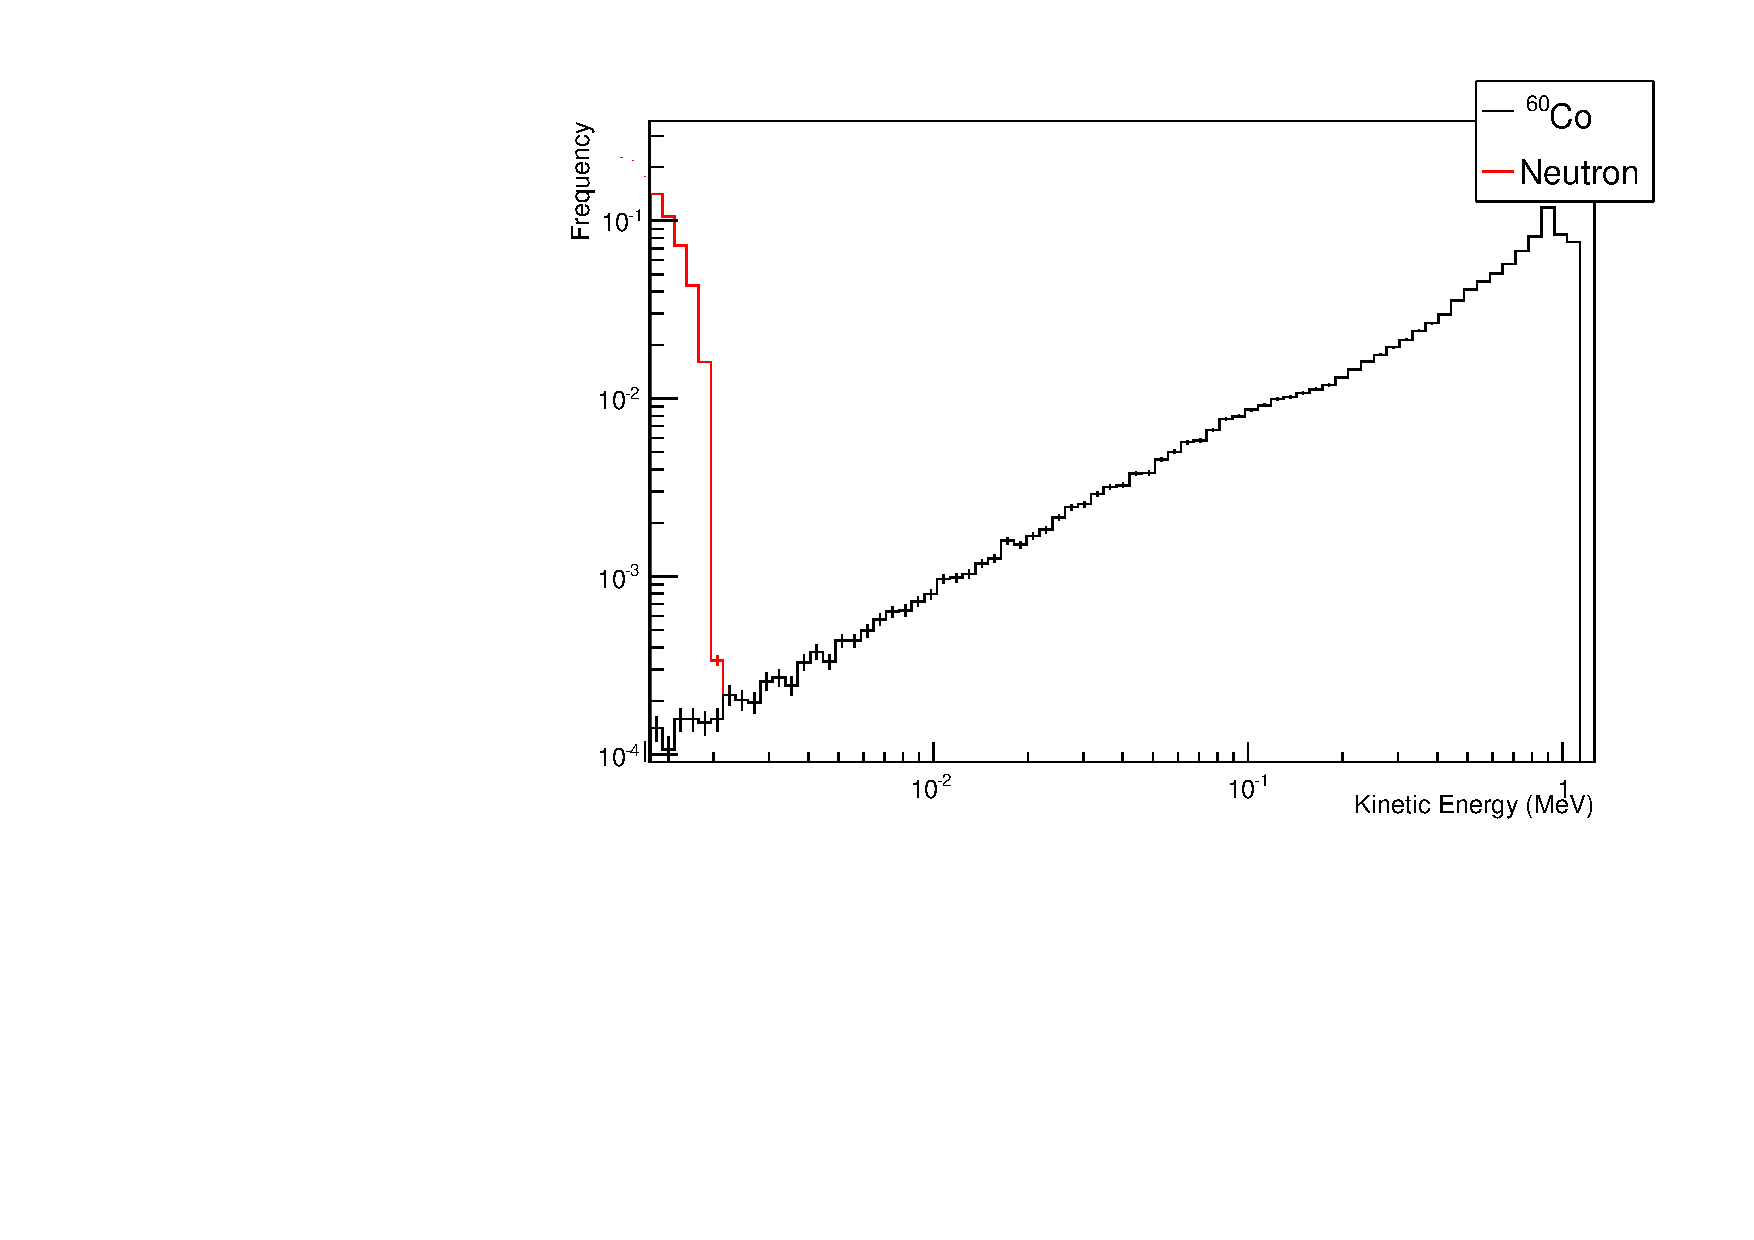
\includegraphics[width=\textwidth]{NGSecElecKinEDist}
    \caption{Simulated Kinetic Energy of Secondary Electrons from Compton Scattering and from \iso[6]{Li} reaction products}
    \label{fig:simKinE}
\end{figure}
\begin{figure*}[ht]
	\centering
	\begin{subfigure}[b]{0.45\textwidth}
    		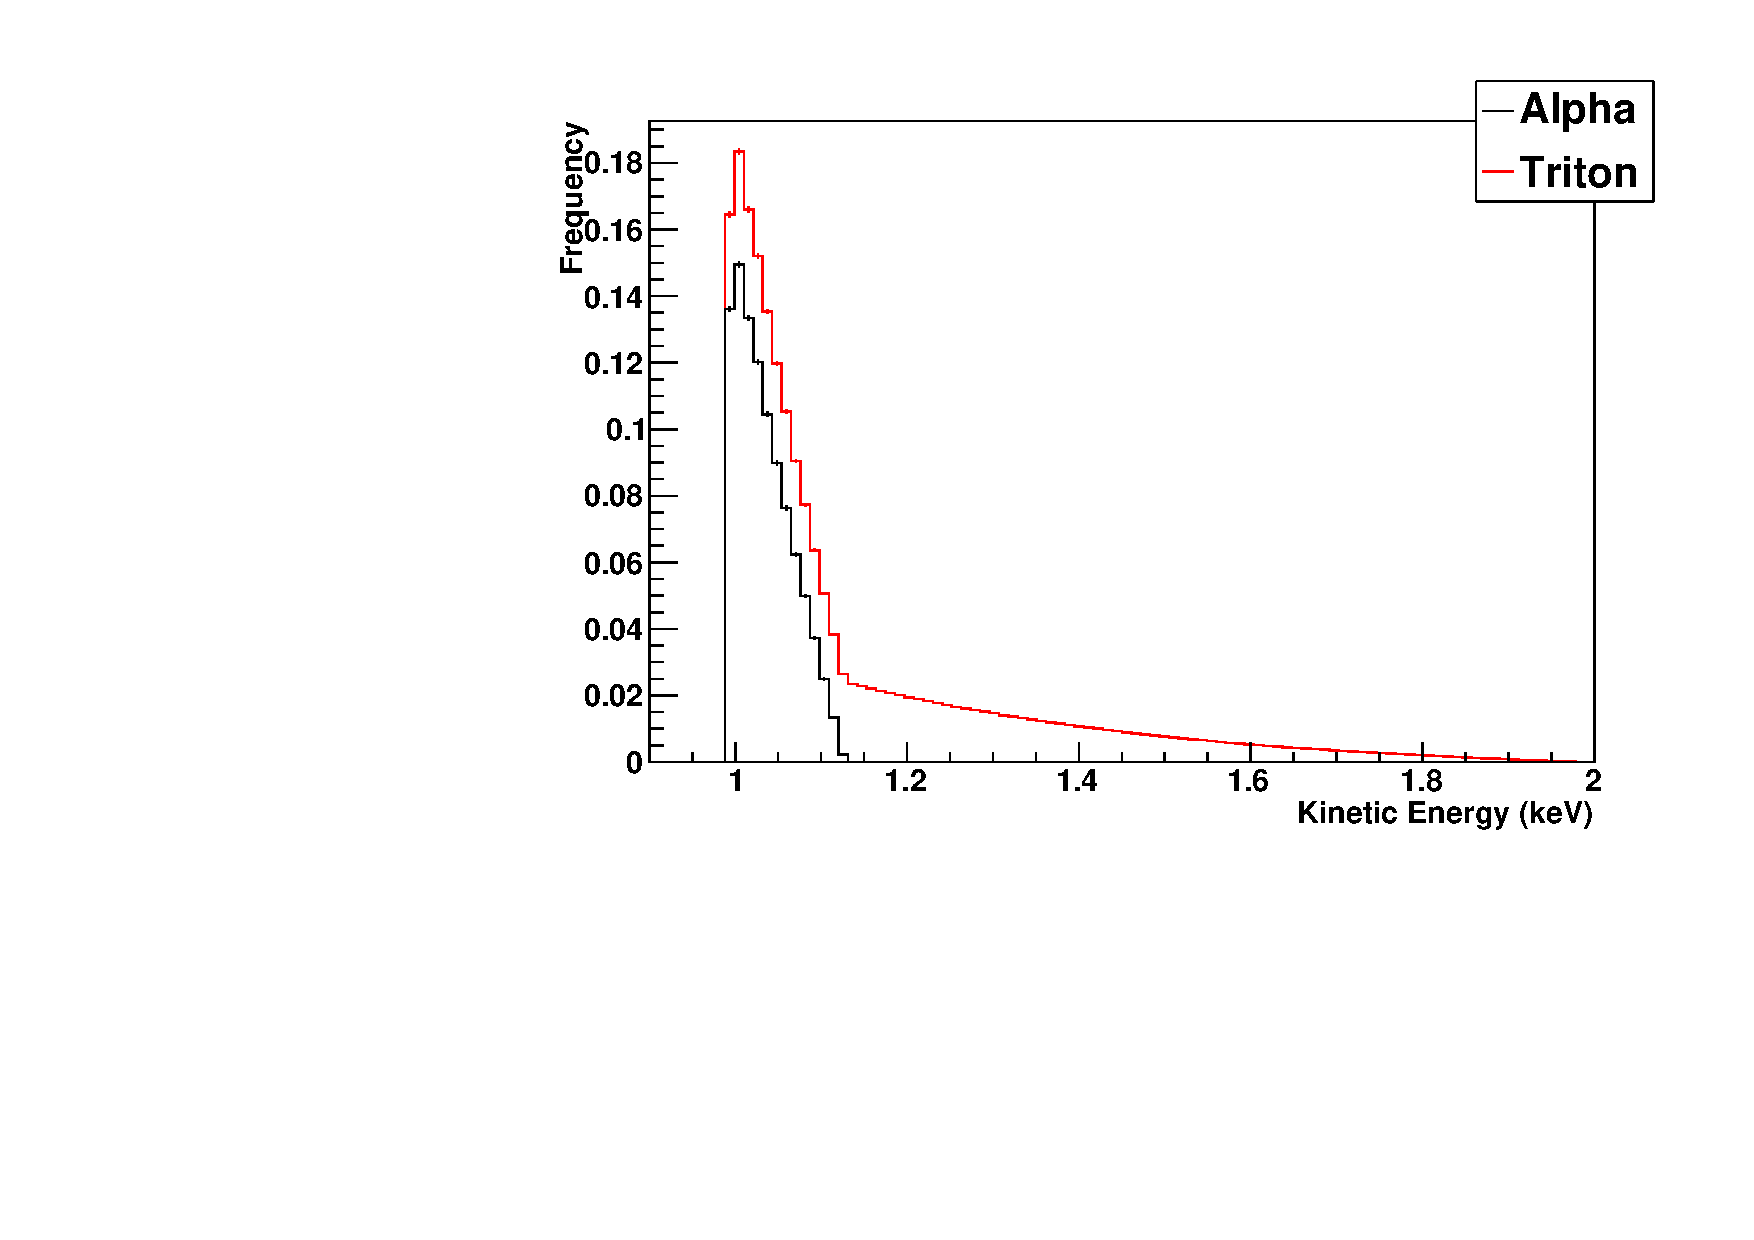
\includegraphics[width=\textwidth]{AlphaTritonSecElecKinEDist}
		\caption{Alpha and Triton Secondary Electron Kinetic Energy Distribution}
	\end{subfigure}%
	~
	\begin{subfigure}[b]{0.45\textwidth}
    		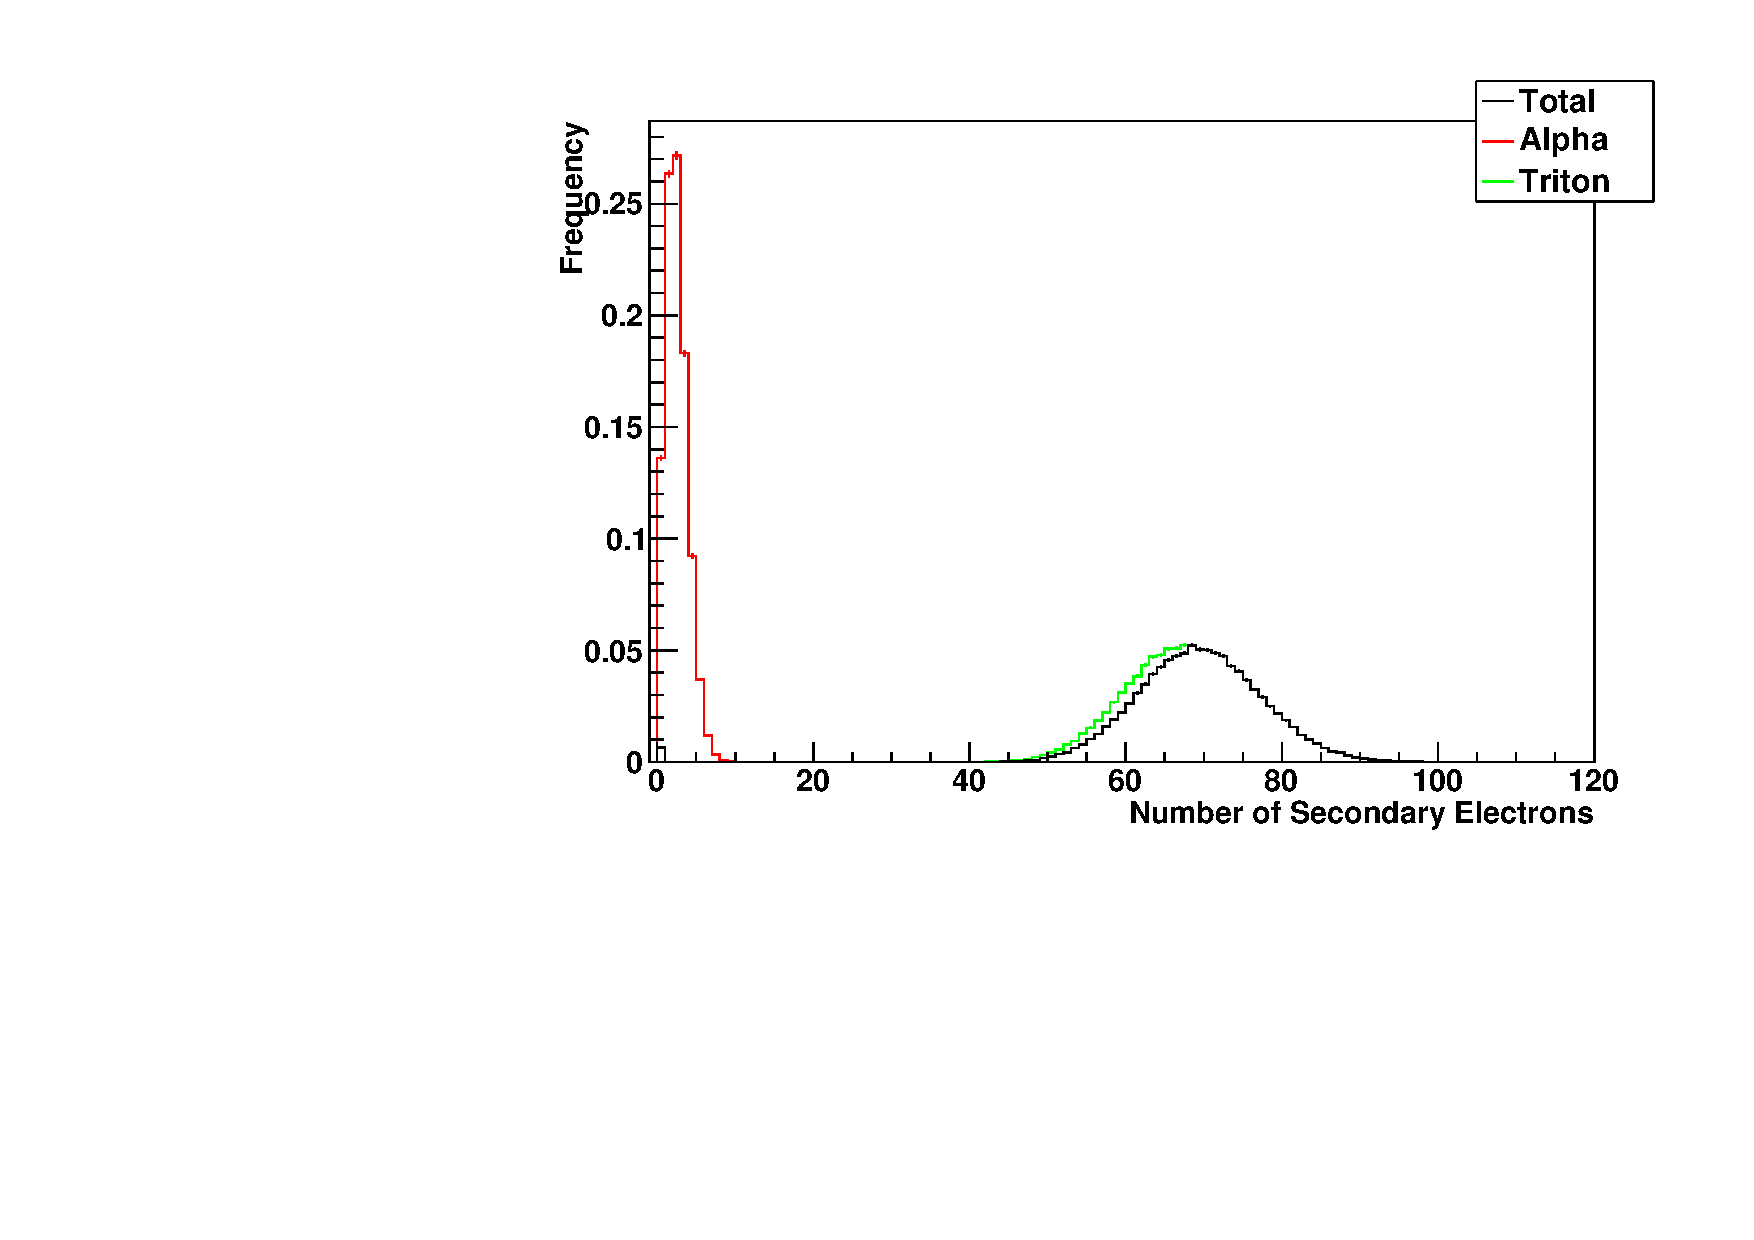
\includegraphics[width=\textwidth]{NeutronNumSecElec}
		\caption{Number of Secondary Electrons Produced Per Neutron Interaction}
	\end{subfigure}%
	\caption{Neutron Reaction Products Secondary Electrons Energies}
	\label{fig:ReacProdDist}
\end{figure*}
%%%%%%%%%%%%%%%%%%%%%%%%%%%%%%%%%%%%%%%%%%%%%%%%%%%%%%%%%%%%%%%%%%%%%%%%%%%
%                                                                         %
%                             CONCLUSIONS                                 %
%                                                                         %
%%%%%%%%%%%%%%%%%%%%%%%%%%%%%%%%%%%%%%%%%%%%%%%%%%%%%%%%%%%%%%%%%%%%%%%%%%%
\section{Conclusions and Future Work}
\label{sec:Conclusions}

The difference in energy deposition between a gamma event in a thin film and a neutron event allows for a pulse height discriminator to be for the discrimination between neutrons and gammas.
GEANT4 Monte Carlo simulations of the energy deposition show that for a \SI{150}{\um} film over 90\% of the reaction product energies from a $\iso[6]{Li}\left(n,t\right)\alpha$ are deposited in the film, but only 3.2\% of the gamma energies from a \iso[60]{Co} decay is deposited.

Future work will focus on the optimization of such a layered detector RPM.
In addition, light transport in layered thin film detectors will be explored.
%%%%%%%%%%%%%%%%%%%%%%%%%%%%%%%%%%%%%%%%%%%%%%%%%%%%%%%%%%%%%%%%%%%%%%%%%%%%

% Bibliography
\bibliography{../Zotero}

\end{document}

